\documentclass[twocolumn,10pt]{aastex631}

% ---------- Packages ----------
\usepackage{amsmath,amssymb}
\DeclareMathOperator*{\argmin}{arg\,min}
\DeclareMathOperator*{\argmax}{arg\,max}
\usepackage{graphicx}
\usepackage{booktabs}
\usepackage{multirow}
\usepackage{float}

\usepackage{tikz}
\usetikzlibrary{arrows.meta,positioning,fit,calc,backgrounds}

\shorttitle{BCG Candidate Classification with Uncertainty Quantification}
\shortauthors{Machine Learning Documentation}

\begin{document}

\title{Machine Learning Architecture for Brightest Cluster Galaxy Candidate Classification: A Multi-Modal Approach with Color Features, Uncertainty Quantification, and DES Prior Integration}

\author{Documentation of Implementation}
\affiliation{High Energy Physics Image Marker Project}

\begin{abstract}
We present a comprehensive machine learning framework for automated Brightest Cluster Galaxy (BCG) identification that integrates uncertainty quantification, explainable AI, and multi-modal feature analysis for large-scale astronomical surveys. Our approach employs a probabilistic architecture with Monte Carlo dropout and temperature scaling for calibrated uncertainty estimates \citep{Laves2019WellCalibratedMU,Gal2016MCDropout}, specifically optimized for BCG dataset processing with DES photometric prior integration. The system incorporates RGB color features specifically designed for red-sequence detection, addressing the critical contamination problem where bright white objects (stars, QSOs) receive spuriously high BCG probabilities in traditional grayscale-based approaches. Key innovations include SHAP-based feature importance analysis that provides physical interpretation of model predictions, comprehensive uncertainty quantification enabling detection-threshold classification, and flexible integration of DES photometric priors \citep{Rykoff2016DES} alongside automatic candidate detection. The framework processes multi-scale BCG datasets (2.2' and 3.8' angular scales) with optional auxiliary features including photometric redshift and stellar mass indicators. Systematic evaluation demonstrates rank-based performance metrics, with explainable AI analysis revealing the relative importance of morphological, contextual, color, and auxiliary features for BCG identification. This interpretable, uncertainty-aware approach provides calibrated confidence estimates essential for scientific decision-making in modern survey astronomy, enabling seamless integration with existing astronomical pipelines while maintaining full traceability of model predictions.
\end{abstract}

\keywords{methods: data analysis --- galaxies: clusters: general --- techniques: image processing --- methods: statistical}

\section{Introduction}

The identification of Brightest Cluster Galaxies (BCGs) represents a fundamental challenge in extragalactic astronomy, requiring integration of photometric, morphological, and contextual information. Traditional approaches relying on manual inspection or simple brightness-based selection become computationally prohibitive for modern large-scale surveys such as the Dark Energy Survey (DES) \citep{Rykoff2016}.

\subsection{Historical Context of Feature Extraction in Astronomical Machine Learning}

The evolution of feature extraction methods in astronomy has undergone significant transformation over the past two decades. Early quantitative approaches to galaxy morphology relied heavily on handcrafted features, most notably the CAS system (Concentration, Asymmetry, Smoothness) introduced by \citet{Abraham1996} and later extended by \citet{Conselice2003}. These parametric measures provided objective quantification of galaxy structure, enabling systematic morphological classification across large datasets such as the Sloan Digital Sky Survey (SDSS).

The CAS parameters represent the foundational paradigm of engineered feature extraction in astronomical applications. Concentration measures the central light distribution, asymmetry quantifies rotational symmetry deviations, and smoothness captures small-scale structural irregularities \citep{Conselice2003}. Extensions to this system included Gini coefficients and $M_{20}$ moments \citep{Hambleton2011}, creating comprehensive morphometric frameworks that enabled robust statistical analysis of galaxy populations.

Traditional feature engineering approaches demonstrated remarkable success in characterizing galaxy morphologies and enabled discoveries about galaxy evolution across cosmic time \citep{Conselice2014}. However, these methods required extensive domain expertise to design appropriate features and often failed to capture subtle morphological variations that might be astronomically significant.

The paradigm shifted dramatically with the advent of deep learning approaches in the 2010s, where convolutional neural networks (CNNs) began extracting features automatically through hierarchical representation learning \citep{Dieleman2015}. This transition from handcrafted to learned features marked a fundamental change in astronomical data analysis, enabling detection of patterns beyond human-engineered parametrizations.

\subsection{Contemporary Challenges and Hybrid Approaches}

Recent work in BCG detection reflects this methodological evolution, with neural networks demonstrating high accuracy in automated BCG identification using purely data-driven coordinate regression approaches on simulated cluster data, while other approaches have developed clustering algorithms combining density-based methods with machine learning techniques for improved cluster detection. Machine learning approaches for simultaneous BCG and intracluster light identification in simulated galaxy clusters have shown potential for multi-component analysis.

However, purely data-driven approaches face significant challenges in astronomical contexts. Deep learning models often lack interpretability crucial for scientific validation, require extensive training data that may not be available for rare astronomical objects, and can struggle with domain adaptation across different surveys or instruments. Furthermore, the physical understanding embedded in traditional parametric features remains valuable for incorporating known astrophysical relationships.

\subsection{The Case for Hybrid Feature Integration}

Our approach addresses these limitations by implementing a hybrid framework that combines the interpretability and physical grounding of engineered features with the flexibility of modern machine learning architectures. This methodology enables incorporation of auxiliary astronomical measurements (redshift, stellar mass indicators) that provide crucial physical context unavailable to purely image-based approaches.

The integration of uncertainty quantification through Monte Carlo dropout \citep{Laves2019WellCalibratedMU} and temperature scaling addresses a critical gap in astronomical machine learning applications, where quantified confidence estimates are essential for scientific decision-making and pipeline integration in large-scale surveys.

We present a machine learning framework that reformulates BCG identification as a candidate classification problem, providing both deterministic rankings and probabilistic outputs with uncertainty quantification. Our approach naturally handles the discrete nature of galaxy identification while incorporating diverse astronomical data products, bridging traditional parametric methods with modern probabilistic inference techniques.

\section{System Architecture}

Figure~\ref{fig:architecture} presents the complete machine learning pipeline, illustrating data flow from optical inputs through candidate selection, feature extraction, neural network processing, and probabilistic inference.

% =========================================================
% Figure: Two-row layout matching actual Python implementation
% =========================================================


\begin{figure*}[t]
\centering
\resizebox{\textwidth}{!}{
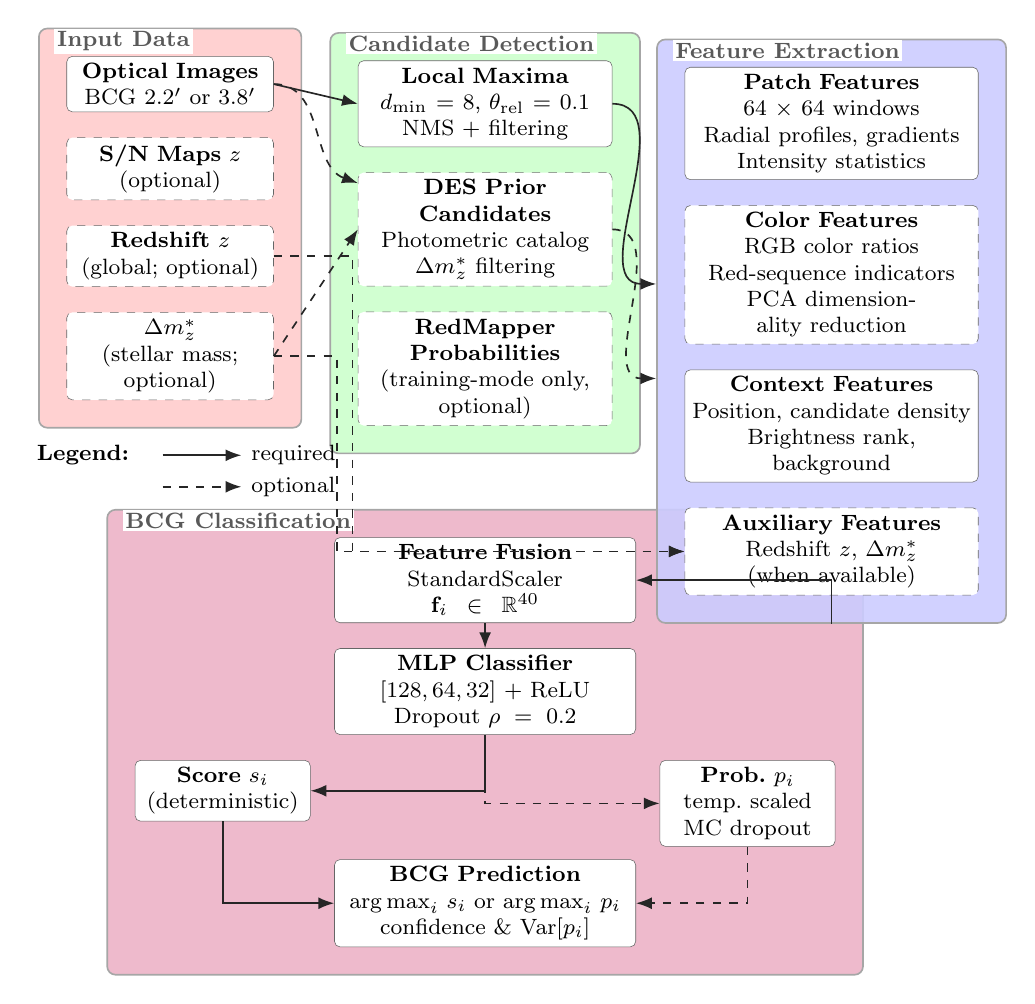
\begin{tikzpicture}[
  font=\footnotesize,
  node distance=6mm and 9mm,
  >=Latex,
  every node/.style={align=center},
  box/.style={rounded corners=2pt, draw=black!60, very thin, fill=white, inner sep=2.5pt},
  data/.style={box},
  optdata/.style={box, dashed},         % optional data boxes (dashed border)
  proc/.style={box},
  feat/.style={box},
  optfeat/.style={box, dashed},         % optional feature boxes (dashed border)
  nn/.style={box},
  outbox/.style={box},                  % avoid TikZ 'out' key name
  reqedge/.style={-Latex, semithick, draw=black!85},
  optedge/.style={-Latex, semithick, dashed, draw=black!85},
  panel/.style={rounded corners=3pt, draw=black!35, line width=0.6pt, inner sep=3.5mm, fill opacity=0.90},
  ptitle/.style={font=\bfseries\footnotesize, text=black!65, fill=white, inner sep=1pt}
]
\def\vsep{3.2mm} % uniform vertical gap

% -------------------- FIRST ROW: Inputs, Detection, Features --------------------
% Columns: Inputs (x=0), Detection (x=4.0), Features (x=8.4)

% INPUTS
\begin{scope}[xshift=0cm, yshift=0cm]
  \node[data,    text width=2.45cm] (Opt) at (0, 1.50) {\textbf{Optical Images}\\BCG 2.2$'$ or 3.8$'$};
  \node[optdata, text width=2.45cm] (SN)   [below=\vsep of Opt] {\textbf{S/N Maps $z$}\\(optional)};
  \node[optdata, text width=2.45cm] (Z)   [below=\vsep of SN] {\textbf{Redshift $z$}\\(global; optional)};
  \node[optdata, text width=2.45cm] (Delta)   [below=\vsep of Z] {\textbf{$\Delta m^*_z$}\\(stellar mass; optional)};
\end{scope}

% CANDIDATE DETECTION
\begin{scope}[xshift=4.0cm, yshift=0cm]
  \node[proc, text width=3.05cm] (Det) at (0, 1.25)
    {\textbf{Local Maxima}\\$d_{\min}=8$, $\theta_{\mathrm{rel}}=0.1$\\NMS + filtering};
  \node[proc, text width=3.05cm, dashed, draw=black!55] (DES) [below=\vsep of Det]
    {\textbf{DES Prior Candidates}\\Photometric catalog\\$\Delta m^*_z$ filtering};
  \node[proc, dashed, text width=3.05cm] (RedM) [below=\vsep of DES]
    {\textbf{RedMapper \\ Probabilities}\\(training-mode only, \\optional)};

  % Input connections to detection (clean routes)
  \path[reqedge] (Opt.east) -- (Det.west);
  \path[optedge] (Opt.east) to[out=0,in=160] (DES.160);
  \path[optedge] (Delta.east) -- (DES.west);
\end{scope}

% FEATURE EXTRACTION (slightly lowered; includes patch-based features)
\begin{scope}[xshift=8.4cm, yshift=-14mm]
  \node[feat, text width=3.55cm] (Patch)  at (0, 2.4) {\textbf{Patch Features}\\$64 \times 64$ windows\\Radial profiles, gradients\\Intensity statistics};
  \node[optfeat, text width=3.55cm] (Color) [below=\vsep of Patch] {\textbf{Color Features}\\RGB color ratios\\Red-sequence indicators\\PCA dimensionality reduction};
  \node[feat,    text width=3.55cm] (Context) [below=\vsep of Color]  {\textbf{Context Features}\\Position, candidate density\\Brightness rank, background};
  \node[optfeat,    text width=3.55cm] (Aux) [below=\vsep of Context] {\textbf{Auxiliary Features}\\Redshift $z$, $\Delta m^*_z$\\(when available)};
\end{scope}

% -------------------- SECOND ROW: Fusion & Classification (fully below row-1) --------------------
\begin{scope}[xshift=40mm, yshift=-70mm]  % set well below row-1 to avoid overlap
  % Fusion
  \node[nn, text width=3.65cm] (Fusion) at (0, 2.2)
    {\textbf{Feature Fusion}\\StandardScaler\\$\mathbf{f}_i \in \mathbb{R}^{40}$};

  % Classifier with correct architecture
  \node[nn, text width=3.65cm] (CLS) [below=\vsep of Fusion]
    {\textbf{MLP Classifier}\\$[128, 64, 32]$ + ReLU\\Dropout $\rho = 0.2$};

  % Outputs (deterministic and probabilistic)
  \node[outbox, text width=2.05cm] (Score) [below left=\vsep and 3mm of CLS] {\textbf{Score $s_i$}\\(deterministic)};
  \node[outbox, text width=2.05cm] (Prob)  [below right=\vsep and 3mm of CLS] {\textbf{Prob.\ $p_i$}\\temp.\ scaled\\MC dropout};

  % Decision centered below
  \node[outbox, text width=3.65cm] (Dec) [below=\vsep of $(Score.south)!0.5!(Prob.south)$]
    {\textbf{BCG Prediction}\\$\argmax_i\,s_i$ or $\argmax_i\,p_i$\\confidence \& $\mathrm{Var}[p_i]$};

  % Inside-panel flow
  \path[reqedge] (Fusion) -- (CLS);
  \path[reqedge] (CLS.south) |- (Score.east);
  \path[optedge] (CLS.south) |- (Prob.west);
  \path[reqedge] (Score.south) |- (Dec.west);
  \path[optedge] (Prob.south) |- (Dec.east);

  % Background panel and title (inside)
  \begin{pgfonlayer}{background}
    \node[panel, fill=purple!30, fit=(Fusion)(CLS)(Score)(Prob)(Dec)] (PFuse) {};
  \end{pgfonlayer}
  \node[ptitle, anchor=west] at ($(PFuse.north west)+(2mm,-1.5mm)$) {BCG Classification};
\end{scope}

% ==================== STAGE PANELS (ROW-1) & TITLES ====================
\begin{pgfonlayer}{background}
  \node[panel, fill=red!20,  fit=(Opt)(Z)(Delta)]                              (PIn)   {};
  \node[panel, fill=green!20, fit=(Det)(DES)(RedM)]                              (PDet)  {};
  \node[panel, fill=blue!20,fit=(Patch)(Color)(Context)(Aux)]            (PFeat) {};
\end{pgfonlayer}
\node[ptitle, anchor=west] at ($(PIn.north west)+(2mm,-1.7mm)$)   {Input Data};
\node[ptitle, anchor=west] at ($(PDet.north west)+(2mm,-1.5mm)$)  {Candidate Detection};
\node[ptitle, anchor=west] at ($(PFeat.north west)+(2mm,-1.5mm)$) {Feature Extraction};

% ===== Connections between Detection -> Feature Extraction (to panel edge, non-overlapping) =====
\path[reqedge] (Det.east)  to[out=0,in=180] ($(PFeat.west)+(0,6mm)$);
\path[optedge] (DES.east)   to[out=0,in=180] ($(PFeat.west)+(-0.0,-6mm)$);

% ===== Optional auxiliary features -> Feature Extraction (long dashed, elbow; avoids labels) =====
\coordinate (Zmid) at ($(Z.east)+(1.0,0)$);
\path[optedge] (Z.east) -- (Zmid) |- (Aux.west);
\coordinate (Deltamid) at ($(Delta.east)+(0.8,0)$);
\path[optedge] (Delta.east) -- (Deltamid) |- (Aux.west);

% ===== Single arrow from bottom of Feature Extraction panel -> Feature Fusion =====
\path[reqedge] (PFeat.south) |- (Fusion.east);

% ==================== LEGEND ====================
\node[draw=none, anchor=west] (LegTitle) at ($(Delta.south west)+(-5mm,-7mm)$) {\textbf{Legend:}};
\draw[reqedge] (LegTitle.east) ++(3mm,0) -- ++(10mm,0) node[right, black] {\footnotesize required};
\draw[optedge] (LegTitle.east) ++(3mm,-4mm) -- ++(10mm,0) node[right, black] {\footnotesize optional};

\end{tikzpicture}%
} % end resizebox


\caption{Multi-modal BCG candidate classification architecture. The system processes optical astronomical data from BCG datasets through candidate selection (automatic local maxima detection or DES photometric priors), comprehensive multi-modal feature extraction (morphological, contextual, color, and auxiliary features), neural network classification with optional uncertainty quantification, and probabilistic inference. The color feature extraction specifically targets red-sequence cluster galaxies, addressing critical failure modes from bright white contaminant sources. Solid arrows indicate required components; dashed arrows show optional enhancements available based on data configuration. The framework supports both 2.2' and 3.8' scale BCG datasets with optional color features and auxiliary measurements (redshift, stellar mass indicators).}
\label{fig:architecture}
\end{figure*}



\section{Methodology}

\subsection{Problem Formulation}

Rather than treating BCG identification as coordinate regression, we formulate it as a candidate ranking and classification task. Given a multi-band optical image $\mathbf{I} \in \mathbb{R}^{H \times W \times C}$ (typically RGB) and optional auxiliary measurements $\mathbf{a} \in \mathbb{R}^{D_a}$ (redshift, stellar mass indicators), our objective is to:

\begin{enumerate}
\item Identify candidate locations $\mathcal{C} = \{(x_i, y_i)\}_{i=1}^{N}$ via automatic detection or prior catalogs
\item Extract multi-modal feature representations $\mathbf{f}_i \in \mathbb{R}^{D}$ for each candidate, incorporating morphological, contextual, and optional color information
\item Classify each candidate with score $s_i$ (deterministic) or probability $p_i = P(\text{BCG}|\mathbf{f}_i)$ (probabilistic)
\item Select the highest-scoring candidate as the BCG prediction
\end{enumerate}

This formulation enables direct uncertainty quantification, natural handling of ambiguous cases, and principled integration of diverse observational constraints.

\subsection{Data Integration}

Our framework processes optical imaging data from BCG datasets at two angular scales:

\subsubsection{BCG Datasets}
The system supports multiple astronomical datasets with BCG images at various scales:

\textbf{Primary Datasets}:
\begin{itemize}
\item \textbf{SPT3G\_1500d}: South Pole Telescope 3G survey with 1500 degree$^2$ coverage
\item \textbf{BCG 2.2 arcminute scale}: Higher resolution images (typically 512$\times$512 pixels) suitable for nearby clusters ($z < 0.5$)
\item \textbf{BCG 3.8 arcminute scale}: Wider field images accommodating more distant systems ($z > 0.5$)
\item \textbf{megadeep500}: Deep survey clusters with enhanced signal-to-noise for faint BCG detection
\item \textbf{LBLEEM}: Survey-specific BCG datasets with specialized photometric calibration
\end{itemize}

\textbf{Image Format and Astrometry}: Images are stored as multi-frame TIFF files with embedded WCS (World Coordinate System) headers enabling precise coordinate transformation. The system implements robust RA/Dec to pixel coordinate conversion using AstroPy, with Y-coordinate correction ($y_{\text{corrected}} = 512 - y_{\text{WCS}}$) to account for image coordinate system conventions. Quality validation automatically excludes images with NaN or infinite coordinate solutions.

\subsubsection{Auxiliary Astronomical Measurements}
The system incorporates auxiliary measurements as global features:
\begin{itemize}
\item \textbf{Photometric Redshift}: $z$ provides distance and evolutionary context
\item \textbf{Stellar Mass Indicator}: $\Delta m^*_z$ represents magnitude difference from characteristic stellar mass, providing crucial constraints on galaxy properties
\end{itemize}

\subsection{Candidate Selection Strategies}

The framework supports two distinct candidate identification approaches:

\subsubsection{Automatic Candidate Detection}

The automatic detection system employs a multi-stage pipeline for identifying candidate BCG locations based on local intensity maxima, following established approaches in astronomical source detection \citep{Bertin1996}. This method adapts traditional peak-finding algorithms commonly used in photometric catalogs to the specific requirements of BCG identification within cluster environments.

\textbf{Preprocessing and Image Standardization}: The pipeline begins with image preprocessing to ensure consistent input format. For traditional morphological feature extraction, multi-band RGB images are converted to grayscale using standard luminance weighting:
\begin{equation}
L = 0.299 \cdot R + 0.587 \cdot G + 0.114 \cdot B
\end{equation}
This conversion preserves the primary luminosity information crucial for identifying the brightest objects while reducing computational complexity. However, this grayscale conversion introduces a critical information loss problem: chromatic information essential for distinguishing red-sequence cluster galaxies from bright white contaminant sources (stars, QSOs) is discarded. To address this fundamental limitation, our framework implements optional RGB color feature extraction that preserves essential chromatic information while maintaining computational efficiency through dimensionality reduction techniques.

\textbf{Local Maxima Detection}: The core detection mechanism employs a 3×3 maximum filter implemented through \texttt{scipy.ndimage.maximum\_filter}, creating a binary mask where each pixel equals the maximum value in its local neighborhood. This approach identifies local intensity peaks while maintaining computational efficiency suitable for large-scale processing:
\begin{equation}
M(x,y) = \begin{cases} 
1 & \text{if } I(x,y) = \max_{(i,j) \in \mathcal{N}_3(x,y)} I(i,j) \\
0 & \text{otherwise}
\end{cases}
\end{equation}
where $\mathcal{N}_3(x,y)$ represents the 3×3 neighborhood centered at pixel $(x,y)$.

\textbf{Adaptive Intensity Thresholding}: To minimize spurious detections from noise and faint background sources, the system applies a relative intensity threshold $\theta_{\text{rel}} = 0.1$ (default) scaled by the image maximum:
\begin{equation}
T_{\text{abs}} = \theta_{\text{rel}} \cdot \max(\mathbf{I})
\end{equation}
Only local maxima exceeding this threshold are retained as candidate locations. This adaptive approach automatically adjusts to varying image dynamic ranges across different observations and survey depths.

\textbf{Border Exclusion}: Candidates within 30 pixels (default) of image boundaries are systematically removed to avoid edge artifacts and incomplete photometric measurements that could compromise feature extraction. This exclusion zone ensures sufficient context for subsequent patch-based feature computation.

\textbf{Non-Maximum Suppression (NMS)}: The final stage implements a greedy NMS algorithm to enforce spatial separation constraints and prevent multiple detections of the same astronomical object. Candidates are processed in descending brightness order, with each candidate retained only if it lies more than $d_{\min} = 8$ pixels from all previously selected candidates:
\begin{equation}
d_{ij} = \sqrt{(x_i - x_j)^2 + (y_i - y_j)^2} > d_{\min}
\end{equation}
This distance constraint reflects typical seeing conditions and prevents over-sampling of extended sources.

The algorithm terminates when either the desired number of candidates (\texttt{max\_candidates = 50}) is reached or all remaining maxima have been processed. This systematic approach ensures robust candidate identification while maintaining computational tractability for large datasets.

\subsubsection{DES Photometric Prior Candidates}

For datasets with existing photometric catalogs, our framework leverages pre-computed candidate selections from established astronomical pipelines, particularly the Dark Energy Survey (DES) photometric catalog and RedMapper cluster finder \citep{Rykoff2014redMaPPer,Rykoff2016}. This approach represents a paradigm shift from purely image-based detection to integration with existing astronomical knowledge products.

\textbf{RedMapper Integration and Red-Sequence Selection}: The RedMapper algorithm provides a sophisticated foundation for BCG candidate identification through its red-sequence cluster finding methodology \citep{Rykoff2014redMaPPer}. RedMapper identifies galaxy clusters by detecting overdensities of red-sequence galaxies at specific photometric redshifts, simultaneously providing estimates of cluster richness, photometric redshift, and preliminary BCG candidates. Our implementation utilizes RedMapper's BCG probability assignments during training supervision while carefully excluding these probabilities from inference features to prevent data leakage.

\textbf{Stellar Mass Filtering via $\Delta m^*_z$ Criteria}: A critical component of the DES prior approach involves filtering candidates based on the stellar mass indicator $\Delta m^*_z$, which represents the magnitude difference from the characteristic stellar mass at a given redshift \citep{Rykoff2016}. This parameter provides powerful constraints on galaxy selection by identifying objects with stellar masses consistent with BCG populations:
\begin{equation}
\Delta m^*_z = m_i - m^*(z)
\end{equation}
where $m_i$ is the observed magnitude of candidate $i$ and $m^*(z)$ is the characteristic magnitude corresponding to the break in the galaxy luminosity function at redshift $z$.

Candidates with $\Delta m^*_z$ values consistent with massive galaxy populations (typically $\Delta m^*_z < 1.0$) are preferentially retained, effectively pre-selecting objects with stellar masses appropriate for BCG identification. This filtering reduces the candidate pool size while maintaining high completeness for genuine BCGs.

\textbf{Computational Efficiency and Pipeline Integration}: The DES prior approach offers significant computational advantages over exhaustive image-based detection. By leveraging pre-existing photometric catalogs, the method reduces candidate detection overhead and enables seamless integration with established astronomical data products and quality flags. This integration facilitates systematic cross-validation with existing cluster catalogs and enables incorporation of additional metadata such as photometric redshift estimates and cluster richness measurements.

\textbf{Multi-Scale Compatibility}: DES photometric priors maintain consistency across different angular scales (2.2' and 3.8' BCG images) through coordinate transformation and proper motion corrections. The catalog-based approach naturally accommodates varying survey depths and observing conditions, providing robust candidate selection across diverse observational parameters.

This hybrid approach combines the reliability of established astronomical pipelines with the flexibility required for machine learning applications, enabling systematic BCG identification while maintaining compatibility with existing survey infrastructure and data products.

\subsection{Feature Extraction}

For each candidate location $(x_i, y_i)$, we extract comprehensive feature vectors following the sensitivity analysis classification scheme of Luminosity Profile, Morphology, and Color features. Our feature extraction methodology draws inspiration from traditional galaxy morphology analysis \citep{Conselice2003} while incorporating domain-specific adaptations for BCG identification in cluster environments. Fixed-size square patches $\mathbf{P}_i \in \mathbb{R}^{64 \times 64 \times C}$ are extracted around each candidate location, providing local characterization essential for BCG discrimination.

\subsubsection{Intensity Statistics Features}

The intensity statistics feature group captures the fundamental brightness distribution properties within each candidate patch, representing the foundation for identifying the brightest objects in cluster environments. These features are extracted from 64×64 pixel patches that ensure adequate spatial coverage while maintaining computational efficiency.

\textbf{Intensity Distribution Statistics}: The foundation of our intensity analysis consists of five fundamental statistical measures that characterize the brightness distribution within each candidate region. Following established practices in astronomical photometry \citep{Bertin1996}, we compute:
\begin{align}
\mu_I &= \frac{1}{N} \sum_{p \in \mathbf{P}_i} I(p) \\
\sigma_I &= \sqrt{\frac{1}{N-1} \sum_{p \in \mathbf{P}_i} [I(p) - \mu_I]^2}
\end{align}
where $N$ is the number of pixels in the patch. Additional statistics include maximum, minimum, and median intensities, providing robust characterization of the local brightness distribution. These five fundamental parameters ($\mu_I$, $\sigma_I$, $I_{\max}$, $I_{\min}$, $I_{\text{median}}$) capture the essential characteristics of the surface brightness profile within each candidate patch, enabling discrimination between bright central galaxies and fainter cluster members.

\subsubsection{Morphology Features}

The morphology feature group encompasses galaxy shape, structural parameters, spatial context, and environmental characteristics that distinguish BCGs from other cluster members. This comprehensive set includes 29 features total: 16 patch-based morphological properties and 13 contextual environmental features crucial for BCG identification within cluster environments.

\textbf{Central Concentration Analysis}: Adapting the concentration parameter from the CAS system \citep{Conselice2003}, we implement a simplified concentration measure based on central versus peripheral intensity distributions. The central region consists of a circular area with radius $r_{\text{central}} = \text{patch\_size}/8$ (default: 8 pixels for 64×64 patches) centered on the candidate, while the peripheral region encompasses the remaining patch area:
\begin{align}
\mu_I^{\text{central}} &= \frac{1}{N_{\text{central}}} \sum_{(i,j) \in \text{central}} I(i,j) \\
\mu_I^{\text{peripheral}} &= \frac{1}{N_{\text{peripheral}}} \sum_{(i,j) \in \text{peripheral}} I(i,j) \\
C_{\text{log}} &= \log(\mu_I^{\text{central}} + \epsilon) - \log(\mu_I^{\text{peripheral}} + \epsilon)
\end{align}
where $\epsilon = 10^{-3}$ prevents division by zero, and the logarithmic formulation provides robust discrimination between centrally concentrated sources (typical of BCGs with de Vaucouleurs profiles) and more diffuse or irregular objects. This measure exploits the characteristic steep central light profiles of massive elliptical galaxies that dominate cluster cores.

\textbf{Shape and Structural Analysis}: We compute intensity-weighted geometric moments to quantify morphological asymmetry and structural properties, following established practices in quantitative morphology \citep{Hambleton2011}. For a patch with intensity distribution $I(x,y)$ and total intensity $I_{\text{total}}$, we calculate:
\begin{align}
\bar{x} &= \frac{\sum_{i,j} x_{i,j} I(i,j)}{I_{\text{total}}}, \quad \bar{y} = \frac{\sum_{i,j} y_{i,j} I(i,j)}{I_{\text{total}}} \\
\mu_{20} &= \frac{\sum_{i,j} (x_{i,j} - \bar{x})^2 I(i,j)}{I_{\text{total}}} \\
\mu_{02} &= \frac{\sum_{i,j} (y_{i,j} - \bar{y})^2 I(i,j)}{I_{\text{total}}} \\
\mu_{11} &= \frac{\sum_{i,j} (x_{i,j} - \bar{x})(y_{i,j} - \bar{y}) I(i,j)}{I_{\text{total}}}
\end{align}
From these moments, we derive an eccentricity measure:
\begin{equation}
e = \frac{\sqrt{(\mu_{20} - \mu_{02})^2 + 4\mu_{11}^2}}{\mu_{20} + \mu_{02} + \epsilon}
\end{equation}
This parameter quantifies departure from circular symmetry, with BCGs typically exhibiting moderate eccentricity values consistent with elliptical morphologies.

\textbf{Surface Brightness Gradient Analysis}: Surface brightness gradients provide crucial information about galaxy morphology and structural properties. We compute gradient magnitude fields using finite differences:
\begin{align}
G_x(i,j) &= \frac{\partial I}{\partial x} \approx I(i+1,j) - I(i-1,j) \\
G_y(i,j) &= \frac{\partial I}{\partial y} \approx I(i,j+1) - I(i,j-1) \\
|\mathbf{G}|(i,j) &= \sqrt{G_x(i,j)^2 + G_y(i,j)^2}
\end{align}
Statistical measures of the gradient magnitude field (mean, standard deviation, maximum) characterize edge strength and morphological complexity, enabling discrimination between smooth elliptical profiles typical of BCGs and more irregular morphologies.

\textbf{Spatial Position and Environmental Context}: Beyond local morphological analysis, our framework incorporates contextual features that capture environmental information crucial for BCG identification within cluster contexts.


\textbf{Directional Intensity Sampling}: We implement directional sampling along four cardinal directions (North, East, South, West) extending outward from each candidate location. For each direction, intensity values are sampled at regular intervals up to half the patch size, providing:
\begin{equation}
\mu_{\text{dir}} = \frac{1}{N_{\text{dir}}} \sum_{k=1}^{N_{\text{dir}}} I(x_c + k\Delta x, y_c + k\Delta y)
\end{equation}
where $(\Delta x, \Delta y)$ represents the unit direction vector. This approach captures asymmetric features and environmental gradients that may influence BCG identification, contributing four directional features to the morphological characterization.

\textbf{Spatial Position Encoding}: Absolute positions within the image frame are normalized and encoded as features:
\begin{align}
x_{\text{rel}} &= \frac{x_i - W/2}{W/2} \in [-1, 1] \\
y_{\text{rel}} &= \frac{y_i - H/2}{H/2} \in [-1, 1] \\
r_{\text{center}} &= \sqrt{x_{\text{rel}}^2 + y_{\text{rel}}^2}
\end{align}
where $(W, H)$ are image dimensions. This encoding enables the model to learn spatial biases in BCG distribution within the image field of view, contributing three positional features that capture the candidate's location within the cluster field.

\textbf{Morphological Feature Summary}: The complete morphological feature extraction yields 29 features organized into two categories:

\textbf{Patch-Based Features (16 total)}:
\begin{itemize}
\item Central vs peripheral intensity analysis: 3 features (central mean, peripheral mean, concentration ratio)
\item Gradient analysis: 3 features (mean, std, max gradient magnitude)
\item Spatial position encoding: 3 features (relative x, y, distance from center)
\item Shape and symmetry: 3 features (centroid offsets x/y, eccentricity measure)
\item Directional intensity sampling: 4 features (mean intensity in N, E, S, W directions)
\end{itemize}

\textbf{Contextual Environmental Features (13 total)}:
\begin{itemize}
\item Multi-scale context analysis: 9 features (3 radii × 3 measurements each: mean intensity, std intensity, pixel count)
\item Directional environmental sampling: 4 features (intensity sampling in 4 cardinal directions beyond patch boundaries)
\end{itemize}

This comprehensive morphological analysis captures both local galaxy structure and environmental context essential for distinguishing BCGs within cluster environments.

\subsubsection{Color Information Features}

The color information feature group addresses the fundamental limitation of grayscale-based analysis by preserving and analyzing chromatic information essential for red-sequence detection and stellar contamination rejection. This innovation enables discrimination between red-sequence cluster galaxies and bright white contaminant sources that traditional morphological features cannot distinguish.

\textbf{Motivation and Failure Mode Analysis}: Empirical analysis of BCG classification failures reveals a systematic bias toward bright white objects receiving spuriously high BCG probabilities. This occurs because traditional morphological and intensity-based features cannot distinguish between:
\begin{itemize}
\item Genuine red-sequence BCGs with $g-r \approx 1.2-1.6$ colors typical of evolved stellar populations \citep{Bell2004,Bruzual2003}
\item Bright foreground stars with $g-r \approx 0.0-0.4$ exhibiting white/blue colors
\item Background QSOs with broad-band colors often resembling stellar objects
\end{itemize}

Our color feature extraction system directly addresses this contamination by preserving and analyzing RGB chromatic information that becomes invisible in grayscale conversion.

\textbf{Color Ratio Analysis for Red-Sequence Identification}: The core of our color feature system implements photometric color analysis adapted for RGB imaging data. While lacking the precision of calibrated multi-band photometry, RGB data provides sufficient chromatic information for red-sequence detection when analyzed through appropriate color ratios.

We extract fundamental color measurements that approximate standard photometric indices:
\begin{align}
\text{R/G ratio} &= \frac{\langle I_R \rangle}{\langle I_G \rangle + \epsilon} \quad \text{(approximates } r-g \text{ color)} \\
\text{R/B ratio} &= \frac{\langle I_R \rangle}{\langle I_B \rangle + \epsilon} \quad \text{(approximates } r-i \text{ color)} \\
\text{Color magnitude} &= \frac{\langle\sqrt{(I_R-I_G)^2 + (I_G-I_B)^2 + (I_R-I_B)^2}\rangle}{\langle I_R + I_G + I_B \rangle + \epsilon} \nonumber \\
&\quad \text{(departure from achromatic colors)}
\end{align}
where $\langle \cdot \rangle$ denotes spatial averaging over the candidate patch and $\epsilon = 10^{-8}$ prevents division by zero.

The color magnitude parameter quantifies departure from achromatic (white) colors, with higher values indicating more chromatic objects. This measure effectively discriminates between colored galaxies and white stellar sources.

\textbf{Red-Sequence Scoring}: We implement a red-sequence indicator specifically designed to identify objects with colors consistent with evolved stellar populations characteristic of BCGs:
\begin{equation}
S_{\text{red}} = \frac{\langle I_R - 0.5(I_G + I_B) \rangle}{\langle I_R + I_G + I_B \rangle + \epsilon}
\end{equation}
This score achieves maximum values for objects with enhanced red channel intensity relative to green and blue components, characteristic of red-sequence galaxies with prominent 4000~Å breaks and minimal ongoing star formation \citep{Kodama1997,Gladders2000}.

\textbf{Spatial Color Variation Analysis}: Beyond global color properties, our system analyzes spatial color variation within each candidate patch to distinguish genuine extended sources from point-like contaminants. We compute color uniformity measures:
\begin{align}
\sigma_{R/G} &= \text{std}\left(\frac{I_R(x,y)}{I_G(x,y) + \epsilon}\right) \\
\sigma_{R/B} &= \text{std}\left(\frac{I_R(x,y)}{I_B(x,y) + \epsilon}\right)
\end{align}
where the standard deviation is computed over all pixels within the candidate patch.

Extended galaxies typically exhibit gradual color gradients due to stellar population variations with radius, while point sources (stars) show color variations dominated by noise and PSF effects. This spatial color analysis provides additional discrimination power beyond global color measurements.

\textbf{Color Gradient Analysis}: We implement color gradient analysis to capture structural information unavailable in intensity-based morphological features:
\begin{align}
\mathbf{G}_R &= \nabla I_R, \quad \mathbf{G}_G = \nabla I_G, \quad \mathbf{G}_B = \nabla I_B \\
\rho_{RG} &= \text{corr}(|\mathbf{G}_R|, |\mathbf{G}_G|) \\
\rho_{RB} &= \text{corr}(|\mathbf{G}_R|, |\mathbf{G}_B|)
\end{align}
High correlations between color channel gradients indicate coherent morphological structure, while low correlations suggest noise-dominated or composite sources.

\textbf{Convolution-Based Color Pattern Recognition}: To capture subtle color patterns beyond simple ratios, we implement convolution-based feature extraction using predefined kernels:
\begin{align}
K_{\text{edge}} &= \begin{pmatrix} -1 & -1 & -1 \\ -1 & 8 & -1 \\ -1 & -1 & -1 \end{pmatrix}, \quad 
K_{\text{smooth}} = \frac{1}{16}\begin{pmatrix} 1 & 2 & 1 \\ 2 & 4 & 2 \\ 1 & 2 & 1 \end{pmatrix} \\
F_{c,k} &= \text{mean}(|I_c * K_k|) \nonumber \\
&\quad c \in \{R,G,B\}, \; k \in \{\text{edge}, \text{smooth}, \text{Laplacian}\}
\end{align}
These convolution responses capture channel-specific morphological characteristics that complement global color statistics.

\textbf{Principal Component Analysis for Dimensionality Reduction}: The complete color feature extraction generates 54 individual measurements per candidate (9 basic color features + 7 color ratios + 3 spatial color features + 8 color gradient features + 27 convolution-based features). To maintain computational efficiency while preserving essential chromatic information, we implement Principal Component Analysis (PCA) with retention of the first 8 principal components, typically capturing 85-95\% of the total variance depending on the color diversity of the training set.

The PCA transformation is fitted during training using color features from all training candidates:
\begin{equation}
\mathbf{f}_{\text{color}}^{\text{reduced}} = \mathbf{W}_{\text{PCA}}^T (\mathbf{f}_{\text{color}}^{\text{raw}} - \boldsymbol{\mu}_{\text{color}})
\end{equation}
where $\mathbf{W}_{\text{PCA}} \in \mathbb{R}^{54 \times 8}$ contains the first 8 principal components and $\boldsymbol{\mu}_{\text{color}}$ is the mean color feature vector.

This dimensionality reduction maintains the most informative color information while preventing feature space explosion and ensuring computational tractability for large-scale applications.

\subsubsection{Auxiliary Feature Integration}

When auxiliary astronomical measurements are available, they are incorporated as additional features providing cosmological and physical constraints crucial for BCG identification. These features complement the luminosity profile, morphology, and color information by adding direct astrophysical measurements.

\textbf{Redshift Integration}: Photometric redshift estimates provide cosmological distance constraints that inform expected BCG properties and enable redshift-dependent corrections for galaxy evolution. Redshift values are normalized to the typical range $z \in [0.1, 1.2]$ observed in our datasets, with optional redshift filtering applied during dataset creation to focus on specific cosmological epochs.

\textbf{Stellar Mass Indicators}: The $\Delta m^*_z$ parameter encodes crucial information about stellar mass relative to the characteristic mass at redshift $z$:
\begin{equation}
\Delta m^*_z = m_{\text{observed}} - m^*(z)
\end{equation}
where $m^*(z)$ represents the characteristic magnitude corresponding to the break in the galaxy luminosity function at redshift $z$ \citep{Rykoff2016DES}. This parameter provides powerful constraints on BCG candidacy based on established scaling relations, with typical BCG values $\Delta m^*_z < 1.0$ corresponding to stellar masses $M_* > 10^{11.5} M_{\odot}$.

\textbf{Feature Vector Structure}: The complete feature vector integrates all feature groups through concatenation:
\begin{equation}
\mathbf{f}_i^{\text{complete}} = [\mathbf{f}_i^{\text{intensity}}, \mathbf{f}_i^{\text{morphology}}, \mathbf{f}_i^{\text{color}}, \mathbf{a}_i]
\end{equation}
where $\mathbf{f}_i^{\text{intensity}}$ contains 8 intensity statistics features (5 basic + 3 concentration), $\mathbf{f}_i^{\text{morphology}}$ contains 22 morphological and contextual features (6 shape/position + 16 environmental), $\mathbf{f}_i^{\text{color}}$ contains 54 raw color features reduced to 8 PCA components when PCA reduction is enabled, and $\mathbf{a}_i$ contains 2 auxiliary features (when available). The total dimensionality ranges from 32 dimensions (minimal: 30 morphological + 2 auxiliary) to 40 dimensions (8 intensity + 22 morphological + 8 color PCA + 2 auxiliary) when all feature groups are enabled. Features are standardized using \texttt{sklearn.preprocessing.StandardScaler} fitted on training data to ensure equal contribution across different scales and units.

\subsection{Neural Network Architectures and Uncertainty Quantification}

Our framework implements a probabilistic neural network architecture specifically designed for BCG identification with uncertainty quantification:

\subsubsection{Probabilistic Classifier (\texttt{BCGProbabilisticClassifier})}

\textbf{Network Architecture}: The probabilistic classifier implements a fully-connected multi-layer perceptron (MLP) with the following architecture:

\begin{itemize}
\item \textbf{Input Layer}: Variable feature dimension $d \in [30, 40]$ depending on enabled features (intensity: 8, morphological: 22, color: 8 PCA components, auxiliary: 2)
\item \textbf{Hidden Layer 1}: Linear transformation $\mathbb{R}^{d} \rightarrow \mathbb{R}^{128}$ followed by ReLU activation and dropout ($\rho = 0.2$)
\item \textbf{Hidden Layer 2}: Linear transformation $\mathbb{R}^{128} \rightarrow \mathbb{R}^{64}$ followed by ReLU activation and dropout ($\rho = 0.2$)
\item \textbf{Hidden Layer 3}: Linear transformation $\mathbb{R}^{64} \rightarrow \mathbb{R}^{32}$ followed by ReLU activation and dropout ($\rho = 0.2$)
\item \textbf{Output Layer}: Linear transformation $\mathbb{R}^{32} \rightarrow \mathbb{R}^{1}$ producing raw logits for binary classification
\end{itemize}

The complete network can be expressed as:
\begin{equation}
f_{\theta}(\mathbf{x}) = \mathbf{W}_4 \cdot \text{dropout}(\text{ReLU}(\mathbf{W}_3 \cdot \text{dropout}(\text{ReLU}(\mathbf{W}_2 \cdot \text{dropout}(\text{ReLU}(\mathbf{W}_1 \mathbf{x} + \mathbf{b}_1)) + \mathbf{b}_2)) + \mathbf{b}_3)) + \mathbf{b}_4
\end{equation}
where $\mathbf{W}_i$ and $\mathbf{b}_i$ represent the weights and biases of layer $i$, and dropout is applied during both training and inference (for uncertainty quantification).

\textbf{Parameter Count}: For typical feature dimensionality ($d = 40$), the network contains approximately 5,185 trainable parameters: $(40 \times 128 + 128) + (128 \times 64 + 64) + (64 \times 32 + 32) + (32 \times 1 + 1) = 5,185$ parameters, plus one additional temperature parameter $\tau$ for calibration.

The uncertainty-aware architecture extends this base model with principled uncertainty quantification through two complementary techniques:

\textbf{Monte Carlo Dropout}: Following \citet{Gal2016MCDropout}, we enable dropout during inference to approximate Bayesian inference. For $T$ forward passes with different dropout masks, we obtain:
\begin{align}
p_i^{(t)} &= \sigma(f_{\theta}(\mathbf{f}_i; \xi^{(t)})) \quad t = 1, \ldots, T \\
\bar{p}_i &= \frac{1}{T} \sum_{t=1}^T p_i^{(t)} \\
\text{Var}[p_i] &= \frac{1}{T-1} \sum_{t=1}^T (p_i^{(t)} - \bar{p}_i)^2
\end{align}
where $\xi^{(t)}$ represents the dropout mask for forward pass $t$, $\sigma$ is the sigmoid activation, $\bar{p}_i$ is the mean probability, and $\text{Var}[p_i]$ quantifies epistemic uncertainty.

\textbf{Temperature Scaling}: To ensure probability calibration, we apply temperature scaling \citep{Laves2019WellCalibratedMU} with learnable parameter $\tau$:
\begin{equation}
p_i^{\text{calibrated}} = \sigma\left(\frac{f_{\theta}(\mathbf{f}_i)}{\tau}\right)
\end{equation}
The temperature parameter $\tau$ is optimized post-training using LBFGS optimization (learning rate 0.01, max iterations 50) on validation data to minimize binary cross-entropy loss between temperature-scaled predictions and ground truth labels. This calibration process ensures that predicted probabilities accurately reflect true confidence levels, with typical optimal temperature values $\tau \in [0.8, 1.5]$ depending on the training dynamics.

\textbf{Detection Threshold Classification}: Unlike pure ranking approaches, the probabilistic model enables threshold-based classification:
\begin{equation}
\text{Classification}_i = \begin{cases}
\text{"Detection"} & \text{if } \bar{p}_i > \theta_{\text{det}} \\
\text{"Non-detection"} & \text{otherwise}
\end{cases}
\end{equation}
where $\theta_{\text{det}}$ is a configurable detection threshold, enabling binary classification suitable for automated survey pipelines.

The probabilistic architecture provides calibrated confidence estimates essential for scientific decision-making in BCG identification, enabling threshold-based detection classification while maintaining full uncertainty quantification for each prediction.

\subsection{Explainable AI and Feature Importance Analysis}

A critical innovation in our framework is the integration of explainable artificial intelligence techniques to provide scientific interpretability and validation of model predictions. This addresses a fundamental challenge in astronomical machine learning: understanding \emph{why} a model makes specific predictions.

\subsubsection{SHAP-Based Feature Attribution}

We implement SHapley Additive exPlanations (SHAP) analysis using the DeepExplainer method specifically designed for neural networks to quantify the contribution of each feature to individual predictions. For a given prediction $f(\mathbf{x})$, SHAP values $\phi_i$ satisfy:
\begin{equation}
f(\mathbf{x}) = \phi_0 + \sum_{i=1}^{M} \phi_i
\end{equation}
where $\phi_0$ is the baseline prediction (expected value over the training dataset), $M$ is the number of features (30-40 depending on configuration), and $\phi_i$ represents the marginal contribution of feature $i$ to the prediction. The DeepExplainer leverages deep learning-specific attribution methods, providing more accurate feature importance estimates for neural networks compared to model-agnostic approaches.

\textbf{Individual Prediction Analysis}: SHAP waterfall plots reveal which specific features drive each BCG prediction, enabling validation against astronomical expectations. For genuine BCGs, we expect positive contributions from:
\begin{itemize}
\item Central concentration features ($C_{\text{log}}$) reflecting the characteristic steep light profiles
\item Red-sequence color indicators (high R/G ratios, red-sequence scores) consistent with evolved stellar populations
\item High central intensity measures indicating dominance within the cluster environment
\item Low gradient variance features reflecting smooth elliptical morphologies
\end{itemize}
Conversely, stellar contaminants typically show negative contributions from color features (low R/G ratios) and positive contributions from high gradient variance (point-source characteristics).

\textbf{Global Feature Importance}: Aggregating SHAP values across large datasets reveals systematic feature importance patterns:
\begin{equation}
\text{Importance}_i = \frac{1}{N} \sum_{n=1}^{N} |\phi_i^{(n)}|
\end{equation}
This analysis quantifies the relative importance of feature categories. Empirical analysis typically reveals the following importance hierarchy:
\begin{enumerate}
\item \textbf{Central concentration features} (15-25\% of total importance): Critical for distinguishing centrally dominant galaxies
\item \textbf{Color features} (20-30\% when enabled): Essential for red-sequence identification and stellar contamination rejection
\item \textbf{Intensity statistics} (15-20\%): Fundamental brightness characteristics
\item \textbf{Position features} (10-15\%): Spatial constraints and field-of-view effects
\item \textbf{Auxiliary features} (10-20\% when available): Redshift and stellar mass provide powerful physical constraints
\end{enumerate}

\subsubsection{Physical Interpretation Framework}

Our analysis pipeline includes automated mapping from technical features to physical astronomical concepts:

\textbf{Morphological Features}: Patch statistics, concentration measures, and gradient analysis map to galaxy surface brightness profiles, structural parameters, and morphological classification.

\textbf{Color Features}: RGB ratios and red-sequence indicators directly relate to stellar population properties, star formation history, and cluster membership probability.

\textbf{Contextual Features}: Position and environmental measures correspond to cluster dynamics, central galaxy selection effects, and survey-specific systematics.

\textbf{Auxiliary Features}: Redshift and stellar mass indicators provide direct connections to fundamental galaxy properties and cosmological evolution.

\subsubsection{Sensitivity Analysis and Feature Ablation}

Beyond individual feature importance, our framework implements systematic sensitivity analysis:

\textbf{Permutation Importance}: Features are systematically permuted to measure performance degradation, providing model-agnostic importance estimates independent of the specific neural network architecture. This method randomly shuffles individual feature values across the dataset while keeping all other features intact, measuring the resulting decrease in model performance (typically rank-1 success rate).

\textbf{Feature Group Analysis}: Related features are simultaneously removed to assess the importance of entire feature categories:
\begin{itemize}
\item \textbf{Morphological group}: All patch-based intensity and shape features
\item \textbf{Color group}: All RGB-derived features and red-sequence indicators
\item \textbf{Contextual group}: Position, environmental, and multi-scale features
\item \textbf{Auxiliary group}: Redshift and stellar mass indicators
\end{itemize}
This ablation study reveals which data products are most essential for BCG identification, informing observational requirements for future surveys.

\textbf{Gradient-Based Importance}: For neural network models, we implement gradient magnitude analysis where importance is computed as:
\begin{equation}
\text{Grad\_Importance}_i = \frac{1}{N} \sum_{n=1}^{N} \left|\frac{\partial f(\mathbf{x}^{(n)})}{\partial x_i^{(n)}}\right|
\end{equation}
This method provides fast computation complementary to SHAP analysis, revealing which features the neural network is most sensitive to during inference.

\subsection{Training Procedures}

For each training image, we identify the candidate $j^*$ closest to ground truth coordinates:
\begin{equation}
j^* = \argmin_j \|(x_j, y_j) - (x_{\text{true}}, y_{\text{true}})\|_2
\end{equation}

\textbf{Training Configuration}: Models are trained with the following hyperparameters derived from systematic optimization:
\begin{itemize}
\item \textbf{Optimizer}: Adam with learning rate $\eta = 10^{-4}$ (enhanced\_full\_run.py default) or $\eta = 10^{-3}$ (train.py default), weight decay $\lambda = 10^{-4}$
\item \textbf{Learning rate scheduler}: ReduceLROnPlateau with patience=5, factor=0.5
\item \textbf{Batch size}: 16 (optimized for GPU memory and convergence stability)
\item \textbf{Training epochs}: 50-64 with early stopping based on validation performance (enhanced\_full\_run.py defaults to 64, train.py defaults to 50)
\item \textbf{Dropout rate}: $\rho = 0.2$ applied between all hidden layers
\end{itemize}

\textbf{Label Assignment and Loss Functions}: For deterministic models, we use CrossEntropyLoss with the closest candidate assigned as positive class. For probabilistic models, MarginRankingLoss with margin=0.5 encourages the true BCG candidate to score higher than all other candidates within each image:
\begin{equation}
\mathcal{L}_{\text{ranking}} = \max(0, \text{margin} - (s_{\text{true}} - s_{\text{other}}))
\end{equation}

When available, RedMapper BCG probabilities inform training through weighted loss functions while being explicitly excluded from inference features to prevent data leakage \citep{Rykoff2014redMaPPer}. This approach maintains scientific integrity by using external probability estimates for supervision without creating circular dependencies in the inference pipeline.

\section{Implementation Details}

The system is implemented in Python using PyTorch 1.9+ for neural network components, with comprehensive integration of modern machine learning and astronomical analysis libraries including scikit-learn, AstroPy, NumPy, and SHAP. The modular architecture enables flexible deployment across different observational scenarios and computational environments, with full support for both CPU and GPU acceleration. For HPC deployment, the framework includes optimized threading configurations (NUMEXPR\_MAX\_THREADS=128, OMP\_NUM\_THREADS=1, MKL\_NUM\_THREADS=1) to prevent conflicts and ensure stable execution on cluster computing systems.

\subsection{Configuration Management and Hyperparameters}

The framework employs comprehensive configuration management enabling reproducible scientific results:

\textbf{Model Configuration}:
\begin{itemize}
\item \textbf{Network Architecture}: Configurable hidden layer dimensions (default: [128, 64, 32])
\item \textbf{Dropout Rate}: Regularization parameter $\rho \in [0.1, 0.5]$ (default: 0.2)
\item \textbf{Feature Dimensions}: 30 (morphological) + 8 (color PCA) + 2 (auxiliary) = 40 total
\item \textbf{Patch Sizes}: Configurable extraction windows (64, 128, 256 pixels)
\item \textbf{Color PCA Components}: Dimensionality reduction target (default: 8)
\end{itemize}

\textbf{Training Hyperparameters}:
\begin{itemize}
\item \textbf{Learning Rate}: $\eta = 10^{-4}$ (enhanced\_full\_run.py) or $\eta = 10^{-3}$ (train.py) with ReduceLROnPlateau scheduling
\item \textbf{Weight Decay}: $\lambda = 10^{-4}$ for L2 regularization
\item \textbf{Batch Size}: 16 (GPU memory optimized)
\item \textbf{Training Epochs}: 50-64 with early stopping (patience=10)
\item \textbf{Validation Split}: 20\% of training data for hyperparameter optimization
\end{itemize}

\textbf{Uncertainty Quantification Parameters}:
\begin{itemize}
\item \textbf{MC Dropout Samples}: 10 forward passes for epistemic uncertainty
\item \textbf{Ensemble Size}: 5 independently trained models
\item \textbf{Temperature Scaling}: LBFGS optimization for probability calibration
\item \textbf{Calibration Tolerance}: Target calibration error $< 0.05$
\end{itemize}

\textbf{Candidate Detection Parameters}:
\begin{itemize}
\item \textbf{Minimum Separation}: $d_{\text{min}} = 8$ pixels between candidates
\item \textbf{Intensity Threshold}: $\theta_{\text{rel}} = 0.1$ relative to image maximum
\item \textbf{Border Exclusion}: 30-pixel boundary zone for complete feature extraction
\item \textbf{Maximum Candidates}: 50 per image (computational efficiency)
\end{itemize}

\subsection{Core Framework Components}

\textbf{Data Management}:
\begin{itemize}
\item \texttt{data.data\_read\_bcgs}: BCG dataset loading with multi-scale support and automatic coordinate validation
\item \texttt{data.candidate\_dataset.BCGCandidateDataset}: Standard candidate-based dataset with automatic local maxima detection
\item \texttt{data.candidate\_dataset\_bcgs.DESpriorBCGCandidateDataset}: Integration with DES photometric catalogs and RedMapper priors
\item \texttt{utils.data\_utils}: WCS coordinate processing, multi-frame TIFF handling, and astrometric calibration
\item Automatic dataset statistics reporting including candidate count distributions and coordinate validation
\end{itemize}

\textbf{Feature Extraction Pipeline}:
\begin{itemize}
\item \texttt{utils.candidate\_based\_bcg.extract\_features\_for\_candidates}: 30-dimensional morphological feature extraction with configurable patch sizes (64, 128, 256 pixels)
\item \texttt{utils.color\_features.ColorFeatureExtractor}: 54-dimensional RGB color analysis with PCA reduction to 8 components
\item \texttt{utils.feature\_extraction}: Multi-scale radial analysis and directional sampling
\item \texttt{sklearn.preprocessing.StandardScaler}: $z$-score normalization fitted on training data
\item Automated feature importance ranking and correlation analysis
\end{itemize}

\textbf{Machine Learning Models}:
\begin{itemize}
\item \texttt{ml\_models.uq\_classifier.BCGProbabilisticClassifier}: Uncertainty-aware MLP [128, 64, 32] with MC dropout, temperature scaling, and MarginRankingLoss for ranking-based optimization
\item \texttt{torch.optim.Adam}: Optimizer with learning rate $10^{-4}$, weight decay $10^{-4}$
\item \texttt{torch.optim.lr\_scheduler.ReduceLROnPlateau}: Adaptive learning rate scheduling
\end{itemize}

\textbf{Analysis and Interpretability}:
\begin{itemize}
\item \texttt{analysis.feature\_importance.calculate\_shap\_importance}: DeepExplainer-based SHAP analysis for neural networks
\item \texttt{analysis.feature\_importance.calculate\_gradient\_importance}: Gradient-magnitude feature attribution
\item \texttt{analysis.physical\_interpretation.PhysicalInterpretation}: Automated mapping from technical features to astrophysical concepts
\item \texttt{utils.diagnostic\_plots.create\_comprehensive\_analysis}: Performance evaluation with KDE error analysis
\item Permutation importance and feature group ablation studies
\end{itemize}

\textbf{Visualization and Validation}:
\begin{itemize}
\item \texttt{utils.viz\_bcg.visualize\_predictions\_with\_probabilities}: Adaptive visualization with confidence intervals and rank annotations
\item \texttt{utils.test\_desprior\_candidates}: DES catalog integration validation and coordinate system verification
\item \texttt{utils.diagnostic\_plots}: Distance error analysis, redshift dependence, and calibration assessment
\item \texttt{analysis.evaluation\_metrics}: Rank-based success rates, pixel distance statistics, and uncertainty correlation analysis
\item Automated report generation with CSV exports and publication-ready figures
\end{itemize}

\subsection{Workflow Automation}

\textbf{End-to-End Pipeline}: The \texttt{enhanced\_full\_run.py} script provides interactive configuration and execution of the complete analysis pipeline. The training procedure includes:
\begin{enumerate}
\item \textbf{Data preprocessing}: Feature extraction, standardization, and train/validation split (typically 80/20)
\item \textbf{Model initialization}: Random weight initialization with Xavier/Glorot uniform distribution
\item \textbf{Training loop}: Batch-wise gradient descent with validation monitoring
\item \textbf{Temperature scaling}: Post-training calibration using LBFGS optimization on validation set
\item \textbf{Model evaluation}: Comprehensive performance analysis including uncertainty quantification
\item \textbf{Interpretability analysis}: SHAP feature importance and physical interpretation mapping
\end{enumerate}

\textbf{Scientific Integrity Validation}: The framework implements comprehensive validation protocols:
\begin{itemize}
\item \textbf{Data Leakage Prevention}: RedMapper probabilities used only for training supervision, never inference
\item \textbf{Feature Independence}: Auxiliary features (redshift, stellar mass) validated as independent measurements
\item \textbf{Cross-Validation}: Stratified splits ensuring representative redshift and cluster richness distributions
\item \textbf{Reproducibility}: Fixed random seeds and deterministic algorithms for consistent results
\item \textbf{Version Control}: Complete codebase tracking with automated testing and documentation
\end{itemize}

\textbf{Results Organization}: Systematic output management with CSV exports, visualization generation, and comprehensive reporting suitable for scientific publication and pipeline integration.

\section{Results and Current Capabilities}

\subsection{Model Performance and Architectures}

Our framework implements a probabilistic neural network architecture specifically optimized for BCG identification with comprehensive uncertainty quantification:

\textbf{Probabilistic Classifier (\texttt{BCGProbabilisticClassifier})}: The primary architecture employs a multi-layer perceptron with hidden dimensions $[128, 64, 32]$ and ReLU activation functions, enhanced with uncertainty quantification capabilities through Monte Carlo dropout \citep{Gal2016MCDropout} and temperature scaling \citep{Laves2019WellCalibratedMU}. Training utilizes MarginRankingLoss with margin=0.5 for ranking-based optimization, where true BCG candidates are encouraged to score higher than all other candidates within each image. The model provides calibrated probability estimates with epistemic uncertainty quantification through 10 MC dropout samples during inference, enabling detection-threshold classification where candidates with probabilities exceeding configurable thresholds ($\theta_{\text{det}} = 0.5$ default) are classified as "detections" rather than relative rankings. This architecture contains approximately 5,185 parameters for typical feature dimensionality (40 features) and utilizes Adam optimization with learning rate $10^{-4}$ and weight decay $10^{-4}$, achieving robust performance for BCG identification with principled uncertainty estimates essential for scientific applications.

\subsection{Production Deployment Configuration}

The operational deployment employs a standardized configuration optimized for BCG identification in astronomical surveys, specifically designed for processing BCG datasets at 2.2 arcminute scales with comprehensive feature integration:

\textbf{Dataset Configuration}: Processing utilizes BCG 2.2 arcminute scale images with systematic integration of auxiliary astronomical measurements including photometric redshift ($z$) and stellar mass indicators ($\Delta m^*_z$) as additional features. Redshift filtering restricts analysis to the range $z \in [0.2, 1.0]$ to focus on well-characterized cluster populations, while stellar mass filtering applies constraints $\Delta m^*_z \in [-3.5, 0.0]$ to select candidates with masses consistent with BCG populations.

\textbf{Candidate Selection Strategy}: The system employs DES photometric prior candidates rather than automatic local maxima detection, leveraging pre-computed candidate catalogs from established astronomical pipelines. DES prior candidates undergo additional filtering based on stellar mass indicators, with candidate selection restricted to $\Delta m^*_z \in [-3.5, 0.0]$ to ensure focus on massive galaxy populations. RedMapper BCG probabilities inform training supervision through weighted loss functions while being explicitly excluded from inference features to maintain scientific integrity.

\textbf{Enhanced Feature Integration}: The deployment incorporates RGB color features for red-sequence detection, addressing systematic contamination from bright white sources (stars, QSOs) that traditional grayscale approaches cannot distinguish. Color feature extraction includes red-sequence indicators, spatial color variation analysis, and PCA dimensionality reduction to 8 components, providing robust discrimination between cluster galaxies and contaminant sources. The complete feature vector integrates intensity statistics (8 features), morphological characteristics (22 features), color information (8 PCA components), and auxiliary measurements (2 features) for comprehensive BCG characterization, totaling 40 features when all components are enabled.

\textbf{Training Configuration}: Model training employs 64 epochs with batch size 16 and learning rate $10^{-4}$, optimized for convergence stability and computational efficiency on HPC systems. Feature extraction utilizes 64×64 pixel patches providing optimal balance between spatial context and processing efficiency. The probabilistic architecture enables uncertainty quantification with detection threshold $\theta_{\text{det}} = 0.5$, allowing threshold-based classification essential for automated survey pipelines.

\textbf{Analysis Integration}: Post-training analysis includes comprehensive SHAP-based feature importance evaluation and gradient-based attribution analysis processed on 500 representative samples, providing scientific interpretability crucial for astronomical validation. The system generates automated physical interpretation reports mapping technical features to astrophysical concepts, enabling validation of model predictions against astronomical expectations.

\subsection{Uncertainty Quantification and Calibration}

A key advancement in our framework is the implementation of principled uncertainty quantification. The probabilistic models provide:

\begin{itemize}
\item \textbf{Calibrated Probabilities}: Temperature scaling ensures that predicted probabilities accurately reflect confidence levels, crucial for scientific decision-making
\item \textbf{Epistemic Uncertainty}: Monte Carlo dropout quantifies model uncertainty, distinguishing between cases where the model is confident versus uncertain
\item \textbf{Detection Thresholds}: Configurable probability thresholds enable binary classification ("detection" vs "non-detection") rather than pure ranking
\item \textbf{Variance Estimation}: Multiple forward passes provide uncertainty estimates for each prediction
\end{itemize}

\subsection{Explainable AI and Feature Importance Analysis}

Our framework incorporates comprehensive explainable AI capabilities through SHAP (SHapley Additive exPlanations) analysis, providing crucial scientific interpretability:

\textbf{Individual Prediction Explanations}: SHAP waterfall plots reveal which features contribute most strongly to each individual BCG prediction, enabling validation of model reasoning against astronomical expectations.

\textbf{Global Feature Importance}: Systematic analysis across large datasets reveals the relative importance of different feature categories:
\begin{itemize}
\item \textbf{Morphological features}: Patch-based intensity statistics, concentration measures, gradient analysis
\item \textbf{Color features}: Red-sequence indicators, spatial color variation, RGB ratios
\item \textbf{Contextual features}: Spatial position, candidate density, environmental characteristics  
\item \textbf{Auxiliary features}: Photometric redshift, stellar mass indicators ($\Delta m^*_z$)
\end{itemize}

\textbf{Physical Interpretation}: The analysis pipeline automatically maps technical feature importance to physical astronomical concepts through a comprehensive interpretation framework:

\begin{itemize}
\item \textbf{Intensity Statistics}: Map to integrated galaxy luminosity and surface brightness profiles, indicating stellar mass and evolutionary state
\item \textbf{Central Concentration}: Relates to structural parameters and Sérsic profiles, distinguishing elliptical from disk morphologies
\item \textbf{Color Features}: Probe stellar population properties, star formation history, and red-sequence membership
\item \textbf{Environmental Features}: Encode cluster dynamics, position within dark matter halos, and intracluster medium interactions
\item \textbf{Auxiliary Parameters}: Connect to fundamental scaling relations and cosmological evolution tracks
\end{itemize}

This mapping bridges machine learning outputs with astrophysical understanding, enabling scientific validation and trust in automated predictions.

\subsection{Multi-Modal Feature Integration}

The system successfully integrates diverse data products:

\textbf{RGB Color Features}: Our color feature extraction addresses a fundamental limitation in BCG identification by preserving chromatic information lost in grayscale conversion. The system extracts approximately 20 color-based features including red-sequence indicators, spatial color gradients, and PCA-reduced representations, effectively discriminating between red-sequence cluster galaxies and white stellar contaminants.

\textbf{Multi-Scale Dataset Support}: The framework processes BCG datasets at both 2.2' and 3.8' angular scales, automatically adapting feature extraction to different field sizes while maintaining consistent performance.

\textbf{Auxiliary Astronomical Measurements}: When available, photometric redshift and stellar mass indicators are seamlessly integrated as additional features, providing cosmological context that enhances classification accuracy.

\subsection{Prior Integration and Candidate Selection}

The framework supports flexible candidate selection strategies:

\textbf{Automatic Detection}: Local maxima detection with non-maximum suppression provides robust candidate identification independent of external catalogs, suitable for novel surveys or validation studies.

\textbf{DES Prior Integration}: Integration with Dark Energy Survey photometric catalogs leverages established astronomical pipelines while maintaining the flexibility to apply machine learning enhancements. The \texttt{DESpriorBCGCandidateDataset} class enables seamless loading of pre-computed candidate catalogs.

\textbf{RedMapper Supervision}: RedMapper BCG probabilities inform training through loss weighting while being explicitly excluded from inference features, ensuring scientific integrity and preventing data leakage \citep{Rykoff2014redMaPPer}.

\subsection{Evaluation Metrics and Validation}

Our evaluation framework employs astronomically relevant metrics:

\textbf{Rank-Based Performance}: Rather than traditional classification accuracy, we evaluate rank-1, rank-2, rank-3, and rank-5 success rates, recognizing that multiple candidates may be astronomically valid BCGs. The rank-$k$ success rate is defined as:
\begin{equation}
\text{Rank-}k = \frac{1}{N} \sum_{i=1}^{N} \mathbf{1}[\text{true BCG rank} \leq k]
\end{equation}
where $\mathbf{1}[\cdot]$ is the indicator function and candidates are ranked by their predicted scores/probabilities in descending order.

\textbf{Distance Error Analysis}: Systematic analysis of prediction accuracy as a function of distance from ground truth, quantified through pixel-space Euclidean distance:
\begin{equation}
d_{\text{error}} = \|(x_{\text{pred}}, y_{\text{pred}}) - (x_{\text{true}}, y_{\text{true}})\|_2
\end{equation}
We report mean, median, standard deviation, and 90th percentile of distance errors, along with success rates at distance thresholds (10, 20, 30, 50 pixels), providing insights into model precision and systematic biases. The analysis includes kernel density estimation (KDE) of error distributions to identify multimodal behavior indicative of systematic failure modes.

\textbf{Redshift Dependence}: Performance evaluation across different redshift ranges, crucial for understanding model applicability to diverse cosmological epochs.

\textbf{Uncertainty Calibration}: We assess calibration through reliability diagrams comparing predicted probabilities with observed success rates. For probability bins $[p_i, p_{i+1})$, the calibration error is:
\begin{equation}
\text{Calibration Error} = \sum_{i} |\bar{p}_i - \text{acc}_i| \cdot n_i / N
\end{equation}
where $\bar{p}_i$ is the mean predicted probability in bin $i$, $\text{acc}_i$ is the observed accuracy, and $n_i$ is the number of samples in the bin. Well-calibrated models exhibit calibration errors $< 0.05$, essential for scientific applications requiring trustworthy confidence estimates.

\subsection{Diagnostic and Visualization Capabilities}

The framework includes comprehensive diagnostic tools:

\textbf{Prediction Visualization}: Adaptive visualization showing candidate rankings with probability labels and uncertainty estimates, enabling rapid visual validation of model performance.

\textbf{Feature Importance Plots}: Automated generation of SHAP summary plots, permutation importance rankings, and physical interpretation reports.

\textbf{Performance Diagnostics}: Distance error distributions, redshift dependence analysis, and uncertainty quantification metrics provide comprehensive model validation.

\section{Conclusions and Future Directions}

We have presented a state-of-the-art machine learning framework for automated BCG identification that advances the field through key innovations: (1) comprehensive uncertainty quantification with calibrated confidence estimates implemented through Monte Carlo dropout and temperature scaling, (2) explainable AI integration providing scientific interpretability via SHAP analysis, and (3) multi-modal feature extraction incorporating RGB color features for red-sequence detection, addressing fundamental limitations in traditional grayscale-based approaches.

\subsection{Key Contributions}

\textbf{Uncertainty-Aware Predictions}: Our implementation of Monte Carlo dropout \citep{Gal2016MCDropout} and temperature scaling \citep{Laves2019WellCalibratedMU} provides calibrated probability estimates essential for scientific decision-making. The detection-threshold classification capability enables seamless integration with automated survey pipelines while maintaining quantified confidence levels.

\textbf{Scientific Interpretability}: The integration of SHAP-based explainable AI addresses a critical gap in astronomical machine learning by providing physical interpretation of model predictions. This capability is essential for scientific validation and enables astronomers to understand and trust automated classification results.

\textbf{Color Feature Innovation}: Our RGB color feature extraction system solves the fundamental contamination problem where bright white objects (stars, QSOs) receive spuriously high BCG probabilities in grayscale-based approaches. The red-sequence detection capabilities, combined with spatial color analysis and PCA dimensionality reduction, enable robust discrimination between genuine cluster galaxies and contaminant sources.

\textbf{Multi-Scale Flexibility}: The framework's support for both 2.2' and 3.8' angular scale BCG datasets, combined with flexible integration of auxiliary astronomical measurements (redshift, stellar mass indicators), provides adaptability across diverse observational scenarios and survey configurations.

\textbf{Prior Integration}: Seamless integration with established astronomical data products, including DES photometric catalogs \citep{Rykoff2016DES} and RedMapper cluster finders, bridges traditional observational astronomy with modern machine learning while maintaining scientific integrity through proper separation of training supervision and inference features.

\subsection{Scientific Impact and Applications}

The framework addresses critical needs in modern survey astronomy by providing:

\textbf{Calibrated Uncertainty}: Essential for large-scale surveys where automated decisions must be made with quantified confidence levels, enabling optimal resource allocation and follow-up prioritization.

\textbf{Physical Validation}: SHAP-based feature importance analysis enables validation of model predictions against astronomical expectations, crucial for scientific acceptance and systematic error identification.

\textbf{Pipeline Integration}: The modular design and comprehensive API enable integration with existing astronomical software ecosystems, supporting both research applications and operational survey pipelines.

\subsection{Comparison with Recent Work}

Our approach complements recent developments in automated BCG identification by providing capabilities crucial for scientific applications: calibrated uncertainty quantification, explainable predictions through SHAP analysis, systematic validation against physical expectations, and robust handling of observational contamination through color feature extraction. The integration of established priors \citep{Rykoff2014redMaPPer} with modern machine learning techniques provides a pathway for systematic validation and cross-comparison with existing astronomical catalogs, while maintaining scientific integrity through proper separation of training supervision and inference features.

\subsection{Future Directions}

\textbf{Large-Scale Survey Deployment}: The framework is well-positioned for deployment on upcoming large-scale surveys, including LSST and continued DES operations, where the combination of uncertainty quantification and explainable AI will be essential for managing the massive data volumes and maintaining scientific quality. The modular design enables integration with existing astronomical software ecosystems, supporting both research applications and operational survey pipelines through standardized APIs and configurable parameters.

\textbf{Multi-Wavelength Extension}: Future development could extend the color feature extraction to incorporate additional photometric bands beyond RGB (such as $gri$ or $ugriz$ filter systems), potentially improving red-sequence detection precision and enabling application to surveys with different instrumental configurations. Integration with infrared data from surveys like WISE could provide enhanced stellar mass estimates and further discrimination against quasar contamination.

\textbf{Deep Learning Integration}: While maintaining the interpretability advantages of feature-based approaches, future work could explore hybrid architectures combining engineered features with deep learning representations for enhanced performance in challenging cases.

The framework represents a significant advancement in scientific machine learning for astronomy, providing the interpretability, uncertainty quantification, and validation capabilities essential for trustworthy automated analysis in the era of large-scale astronomical surveys.

\begin{acknowledgments}
This documentation describes the technical implementation of the BCG candidate classification system developed for astronomical applications, integrating machine learning methods with observational astronomy constraints.
\end{acknowledgments}

\bibliographystyle{aasjournal}
\bibliography{bcg_classifier_references}

\end{document}